\subsection{Interfaces}
\subsubsection{Assignation des interfaces}
Aucune interface ne doit être présente sur le serveur sans être assignée. Sur ce cluster, trois interfaces doivent être présentes :
\begin{itemize}
    \item \textbf{WAN}, l'interface directement connectée au routeur fournissant l'accès à Internet
    \item \textbf{DMZ}, l'interface connectée aux équipements présents en DMZ
    \item \textbf{FWLHA}, l'interface permettant aux pare-feu en cluster de communiquer ensemble, notamment en synchronisant les états et les configurations
\end{itemize}

\begin{warning}
    L'interface FWLHA doit idéalement être une connexion directe entre les équipements. En cas d'impossibilité, elle doit être sur un VLAN dédié et isolé, puisqu'elle fait circuler toutes les configurations et les états du cluster.
\end{warning}

\subsubsection{Interface WAN}
\begin{tip}
    Dans le cadre du projet, l'interface WAN sera configurée en DHCP, le routeur Internet fournissant les adresses IP dynamiquement.
\end{tip}

\begin{itemize}
    \item Activer l'interface (figure \ref{fig:04-configuration-interfaces-01})
    \item Nommer l'interface (figure \ref{fig:04-configuration-interfaces-01})
    \item Configurer l'adressage IPv4 (figure \ref{fig:04-configuration-interfaces-01})
    \item Configurer l'adressage IPv6 (figure \ref{fig:04-configuration-interfaces-01})
    \item Autoriser les adresses privées et de loopback (figure \ref{fig:04-configuration-interfaces-02})
    \item Bloquer le trafic bogon (adresses IP réservées mais ne respectant pas la RFC 1918\footnote{\url{https://datatracker.ietf.org/doc/html/rfc1918}} ou non-assignées) (figure \ref{fig:04-configuration-interfaces-02})
    \item Appliquer les changements
\end{itemize}

\begin{figure}[H]
    \centering
    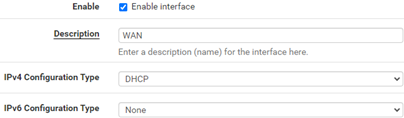
\includegraphics[width=0.7\textwidth]{04-Configuration/Images/04-configuration-interfaces-01.png}
    \caption{Configuration - Interfaces - WAN - Configuration générale}
    \label{fig:04-configuration-interfaces-01}
\end{figure}

\begin{tip}
    Dans le cadre du projet, le routeur opérateur fournit une adresse IP privée, impliquant la nécessité de permettre les adresses IP privées et de loopbacks à communiquer.
\end{tip}

\begin{figure}[H]
    \centering
    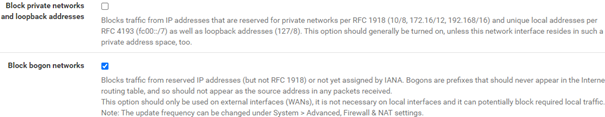
\includegraphics[width=1.0\textwidth]{04-Configuration/Images/04-configuration-interfaces-02.png}
    \caption{Configuration - Interfaces - WAN - Réseaux réservés}
    \label{fig:04-configuration-interfaces-02}
\end{figure}

\subsubsection{Interface DMZ}
\begin{itemize}
    \item Activer l'interface (figure \ref{fig:04-configuration-interfaces-03})
    \item Nommer l'interface (figure \ref{fig:04-configuration-interfaces-03})
    \item Configurer l'adressage IPv4 (figure \ref{fig:04-configuration-interfaces-03})
    \item Désactiver l'adressage IPv6 (figure \ref{fig:04-configuration-interfaces-03})
    \item Définir l'adresse IPv4 et son masque de sous-réseau (figure \ref{fig:04-configuration-interfaces-04})
    \item Autoriser les adresses privées et de loopback (figure \ref{fig:04-configuration-interfaces-05})
    \item Autoriser le trafic bogon (figure \ref{fig:04-configuration-interfaces-05})
    \item Appliquer les changements
\end{itemize}

\begin{figure}[H]
    \centering
    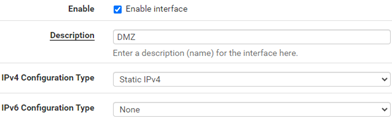
\includegraphics[width=0.7\textwidth]{04-Configuration/Images/04-configuration-interfaces-03.png}
    \caption{Configuration - Interfaces - DMZ - Configuration générale}
    \label{fig:04-configuration-interfaces-03}
\end{figure}

\begin{figure}[H]
    \centering
    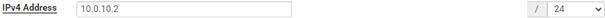
\includegraphics[width=1.0\textwidth]{04-Configuration/Images/04-configuration-interfaces-04.png}
    \caption{Configuration - Interfaces - DMZ - Adresse IPv4}
    \label{fig:04-configuration-interfaces-04}
\end{figure}

\begin{figure}[H]
    \centering
    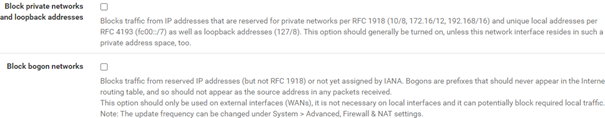
\includegraphics[width=1.0\textwidth]{04-Configuration/Images/04-configuration-interfaces-05.png}
    \caption{Configuration - Interfaces - DMZ - Réseaux réservés}
    \label{fig:04-configuration-interfaces-05}
\end{figure}

\subsubsection{Interface FWLHA}
\begin{itemize}
    \item Activer l'interface (figure \ref{fig:04-configuration-interfaces-06})
    \item Nommer l'interface (figure \ref{fig:04-configuration-interfaces-06})
    \item Configurer l'adressage IPv4 (figure \ref{fig:04-configuration-interfaces-06})
    \item Désactiver l'adressage IPv6 (figure \ref{fig:04-configuration-interfaces-06})
    \item Définir l'adresse IPv4 et son masque de sous-réseau (figure \ref{fig:04-configuration-interfaces-07})
    \item Autoriser les adresses privées et de loopback (figure \ref{fig:04-configuration-interfaces-08})
    \item Autoriser le trafic bogon (figure \ref{fig:04-configuration-interfaces-08})
    \item Appliquer les changements
\end{itemize}

\begin{figure}[H]
    \centering
    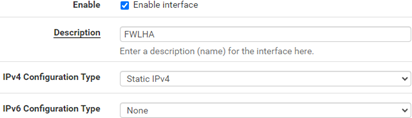
\includegraphics[width=0.7\textwidth]{04-Configuration/Images/04-configuration-interfaces-06.png}
    \caption{Configuration - Interfaces - FWLHA - Configuration générale}
    \label{fig:04-configuration-interfaces-06}
\end{figure}

\begin{figure}[H]
    \centering
    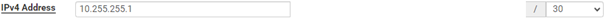
\includegraphics[width=1.0\textwidth]{04-Configuration/Images/04-configuration-interfaces-07.png}
    \caption{Configuration - Interfaces - FWLHA - Adresse IPv4}
    \label{fig:04-configuration-interfaces-07}
\end{figure}

\begin{figure}[H]
    \centering
    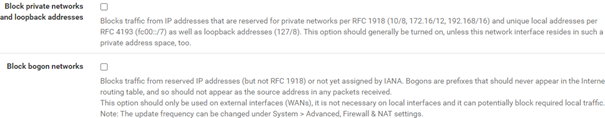
\includegraphics[width=1.0\textwidth]{04-Configuration/Images/04-configuration-interfaces-08.png}
    \caption{Configuration - Interfaces - FWLHA - Réseaux réservés}
    \label{fig:04-configuration-interfaces-08}
\end{figure}
